%======================================================================
% APPENDIX: ARM Architecture and Assembly Language
%
% Target audience: Students who have completed the C appendix and want
% to understand what happens "under the hood" on the STM32 processor
%======================================================================

\chapter{ARM Architecture and Assembly Language}
\label{app:arm-assembly}
\index{ARM architecture|(}
\index{assembly language|(}

\section{Introduction: Why Understand Assembly?}

You will rarely write assembly language directly. Modern compilers generate efficient machine code, and writing assembly by hand is error-prone and time-consuming. So why learn it?

\begin{itemize}
    \item \textbf{Debugging crashes}: When your quadrotor crashes (the software kind), the fault handler gives you register values and a program counter. Understanding assembly lets you trace back to the C code that caused the fault.

    \item \textbf{Understanding timing}: When you need to know exactly how long a piece of code takes, you need to count instructions and their cycle costs.

    \item \textbf{Optimizing critical loops}: The attitude control inner loop runs 1000 times per second. Understanding what the compiler generates helps you write C that compiles to efficient assembly.

    \item \textbf{Hardware interaction}: Startup code, interrupt handlers, and context switches often require assembly.
\end{itemize}

\begin{keyidea}[title=Reading vs. Writing Assembly]
The goal is to \textbf{read} assembly, not write it. When you see a crash dump or disassembly listing, you should be able to understand what the code is doing and trace it back to your C source.
\end{keyidea}

\subsection{The Compilation Pipeline}

Your C code goes through several transformations before running on the processor:

\begin{center}
\begin{tikzpicture}[node distance=2cm, auto,
    block/.style={rectangle, draw, minimum width=2.5cm, minimum height=1cm, align=center}]

    \node[block] (c) {C Source\\(\texttt{.c})};
    \node[block, right=of c] (asm) {Assembly\\(\texttt{.s})};
    \node[block, right=of asm] (obj) {Object\\(\texttt{.o})};
    \node[block, right=of obj] (elf) {Executable\\(\texttt{.elf})};

    \draw[->] (c) -- node[above] {\small compile} (asm);
    \draw[->] (asm) -- node[above] {\small assemble} (obj);
    \draw[->] (obj) -- node[above] {\small link} (elf);
\end{tikzpicture}
\end{center}

\begin{enumerate}
    \item \textbf{Compilation}: The compiler (\texttt{arm-none-eabi-gcc}) translates C to assembly
    \item \textbf{Assembly}: The assembler converts assembly to machine code (object file)
    \item \textbf{Linking}: The linker combines object files and resolves addresses
\end{enumerate}

You can examine the assembly output at any stage:
\begin{lstlisting}[language=bash]
# Generate assembly from C (human-readable)
arm-none-eabi-gcc -S -O2 controller.c -o controller.s

# Disassemble object file
arm-none-eabi-objdump -d controller.o

# Disassemble with source intermixed
arm-none-eabi-objdump -d -S firmware.elf > firmware.lst
\end{lstlisting}

%======================================================================
\section{The STM32F4 and ARM Cortex-M4 Architecture}
%======================================================================

The Crazyflie 2.x uses the \textbf{STM32F405RG}\index{STM32F405} microcontroller, which contains an ARM Cortex-M4\index{ARM Cortex-M4} processor core.

\subsection{STM32F405 Overview}

\begin{center}
\begin{tabular}{ll}
\toprule
\textbf{Feature} & \textbf{Specification} \\
\midrule
Core & ARM Cortex-M4F (with FPU) \\
Clock speed & Up to 168 MHz \\
Flash memory & 1 MB (program storage) \\
SRAM & 192 KB (runtime data) \\
FPU & Single-precision hardware floating point \\
Instruction set & Thumb-2 (16/32-bit mixed) \\
Pipeline & 3-stage (Fetch, Decode, Execute) \\
Interrupts & NVIC with 82 maskable channels \\
\bottomrule
\end{tabular}
\end{center}

\subsection{Memory Map}

The Cortex-M4 has a 32-bit address space (4 GB), but only portions are used:

\begin{center}
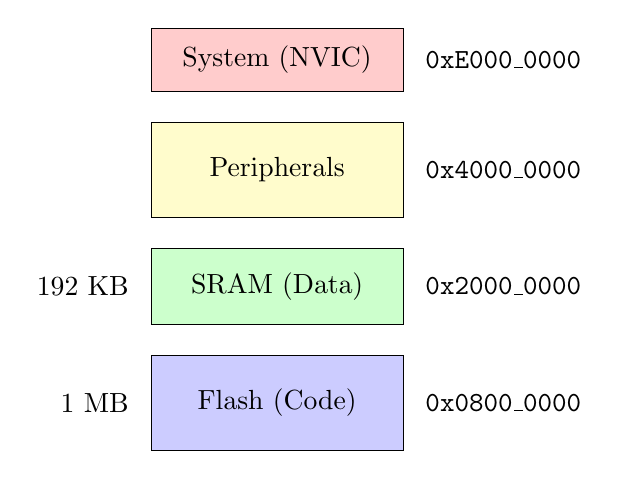
\begin{tikzpicture}[scale=0.8]
    % Memory regions
    \draw[fill=blue!20] (0,0) rectangle (4,1.5);
    \node at (2,0.75) {Flash (Code)};
    \node[right] at (4.2,0.75) {\texttt{0x0800\_0000}};

    \draw[fill=green!20] (0,2) rectangle (4,3.2);
    \node at (2,2.6) {SRAM (Data)};
    \node[right] at (4.2,2.6) {\texttt{0x2000\_0000}};

    \draw[fill=yellow!20] (0,3.7) rectangle (4,5.2);
    \node at (2,4.45) {Peripherals};
    \node[right] at (4.2,4.45) {\texttt{0x4000\_0000}};

    \draw[fill=red!20] (0,5.7) rectangle (4,6.7);
    \node at (2,6.2) {System (NVIC)};
    \node[right] at (4.2,6.2) {\texttt{0xE000\_0000}};

    % Size annotations
    \node[left] at (-0.2,0.75) {1 MB};
    \node[left] at (-0.2,2.6) {192 KB};
\end{tikzpicture}
\end{center}

\begin{itemize}
    \item \textbf{Flash} (\texttt{0x0800\_0000}): Your compiled code lives here. Read-only during execution.
    \item \textbf{SRAM} (\texttt{0x2000\_0000}): Variables, stack, and heap. Read-write.
    \item \textbf{Peripherals} (\texttt{0x4000\_0000}): Timer registers, GPIO, SPI, I2C, etc.
    \item \textbf{System} (\texttt{0xE000\_0000}): NVIC (interrupt controller), SysTick timer, debug registers.
\end{itemize}

\subsection{Cortex-M4 Features for Real-Time Control}

\textbf{Hardware Floating-Point Unit (FPU)}\index{FPU (Floating-Point Unit)}:
\begin{itemize}
    \item Single-precision (32-bit) operations in hardware
    \item Most operations complete in 1 cycle
    \item Division and square root take 14 cycles
    \item Without FPU, floating-point would require ~100 cycles per operation
\end{itemize}

\textbf{Nested Vectored Interrupt Controller (NVIC)}\index{NVIC (Nested Vectored Interrupt Controller)}:
\begin{itemize}
    \item Handles sensor data ready, timer events, communication
    \item 12-cycle interrupt latency (deterministic)
    \item Priority levels allow critical interrupts to preempt less critical ones
\end{itemize}

\textbf{SysTick Timer}:
\begin{itemize}
    \item 24-bit countdown timer
    \item Used by FreeRTOS for task scheduling
    \item Typically configured for 1 ms ticks
\end{itemize}

%======================================================================
\section{ARM Registers}
\index{registers!ARM}
%======================================================================

The Cortex-M4 has 16 general-purpose registers (R0--R15) plus special registers.

\subsection{General-Purpose Registers}

\begin{center}
\begin{tabular}{llp{7cm}}
\toprule
\textbf{Register} & \textbf{Alias} & \textbf{Purpose} \\
\midrule
R0--R3 & --- & Arguments and return value. R0 holds return value. Caller-saved (may be overwritten by called functions). \\
R4--R11 & --- & Local variables. Callee-saved (function must preserve these). \\
R12 & IP & Intra-procedure scratch register. \\
R13 & SP & Stack Pointer. Points to top of stack. \\
R14 & LR & Link Register. Holds return address after BL instruction. \\
R15 & PC & Program Counter. Address of next instruction. \\
\bottomrule
\end{tabular}
\end{center}

\begin{keyidea}[title=Caller-Saved vs. Callee-Saved]
\begin{itemize}
    \item \textbf{Caller-saved} (R0--R3, R12): If you need these values after a function call, save them yourself before calling.
    \item \textbf{Callee-saved} (R4--R11): Functions must restore these before returning. If a function uses R4, it must save and restore it.
\end{itemize}
This convention allows efficient function calls---only registers that are actually used need to be saved.
\end{keyidea}

\subsection{Special Registers}

\begin{center}
\begin{tabular}{lp{9cm}}
\toprule
\textbf{Register} & \textbf{Purpose} \\
\midrule
xPSR & Program Status Register. Contains condition flags (N, Z, C, V), interrupt status, and execution state. \\
PRIMASK & Interrupt mask. Setting bit 0 disables all interrupts (except NMI and HardFault). \\
BASEPRI & Base priority mask. Disables interrupts below a certain priority level. \\
CONTROL & Controls stack pointer selection and privilege level. \\
\bottomrule
\end{tabular}
\end{center}

\subsection{Condition Flags}

The condition flags in xPSR are set by comparison and arithmetic instructions:

\begin{center}
\begin{tabular}{clp{7cm}}
\toprule
\textbf{Flag} & \textbf{Name} & \textbf{Meaning} \\
\midrule
N & Negative & Result was negative (bit 31 = 1) \\
Z & Zero & Result was zero \\
C & Carry & Unsigned overflow occurred \\
V & Overflow & Signed overflow occurred \\
\bottomrule
\end{tabular}
\end{center}

\begin{example}[Flag Setting]
\begin{lstlisting}[language=arm]
    MOV   R0, #5
    MOV   R1, #3
    CMP   R0, R1      @ Computes R0 - R1, sets flags
                      @ Result = 2: N=0 (positive), Z=0 (not zero)

    SUBS  R2, R1, R0  @ R2 = R1 - R0 = 3 - 5 = -2
                      @ N=1 (negative), Z=0, C=0 (borrow)
\end{lstlisting}
\end{example}

\subsection{FPU Registers}

The Cortex-M4F has 32 single-precision floating-point registers:

\begin{center}
\begin{tabular}{llp{7cm}}
\toprule
\textbf{Registers} & \textbf{Convention} & \textbf{Purpose} \\
\midrule
S0--S15 & Caller-saved & Arguments, return value (S0), scratch \\
S16--S31 & Callee-saved & Must be preserved across function calls \\
FPSCR & --- & FPU Status and Control Register (flags, rounding mode) \\
\bottomrule
\end{tabular}
\end{center}

Floating-point arguments are passed in S0, S1, S2, ... and the return value is in S0.

%======================================================================
\section{Memory Model and Addressing}
%======================================================================

\subsection{Byte Ordering: Little-Endian}

ARM Cortex-M uses \textbf{little-endian} byte ordering: the least significant byte is stored at the lowest address.

\begin{center}
\begin{tabular}{c|c|c|c|c}
\multicolumn{5}{c}{32-bit value \texttt{0x12345678} at address \texttt{0x2000\_0000}} \\
\hline
Address & +0 & +1 & +2 & +3 \\
\hline
Content & \texttt{78} & \texttt{56} & \texttt{34} & \texttt{12} \\
\hline
\end{tabular}
\end{center}

\subsection{Alignment}

Memory accesses should be \textbf{aligned} to their natural boundaries:
\begin{itemize}
    \item 32-bit (word): Address divisible by 4
    \item 16-bit (halfword): Address divisible by 2
    \item 8-bit (byte): Any address
\end{itemize}

\begin{warningbox}[title=Alignment Faults]
Unaligned 32-bit access (e.g., loading a word from address \texttt{0x2000\_0001}) causes a \textbf{Usage Fault} on Cortex-M4. This is a common cause of crashes when casting pointers incorrectly:
\begin{lstlisting}[language=C]
uint8_t buffer[10];
uint32_t* ptr = (uint32_t*)&buffer[1];  // Unaligned!
uint32_t value = *ptr;  // CRASH: UsageFault
\end{lstlisting}
\end{warningbox}

\subsection{Load and Store Instructions}

ARM is a \textbf{load-store architecture}: arithmetic operates only on registers. Data must be loaded from memory into registers, processed, then stored back.

\begin{center}
\begin{tabular}{llp{6cm}}
\toprule
\textbf{Instruction} & \textbf{Example} & \textbf{Meaning} \\
\midrule
LDR & \texttt{LDR R0, [R1]} & Load word: R0 = mem[R1] \\
LDRH & \texttt{LDRH R0, [R1]} & Load halfword (16-bit, zero-extend) \\
LDRB & \texttt{LDRB R0, [R1]} & Load byte (8-bit, zero-extend) \\
LDRSB & \texttt{LDRSB R0, [R1]} & Load byte (sign-extend) \\
STR & \texttt{STR R0, [R1]} & Store word: mem[R1] = R0 \\
STRH & \texttt{STRH R0, [R1]} & Store halfword \\
STRB & \texttt{STRB R0, [R1]} & Store byte \\
\bottomrule
\end{tabular}
\end{center}

\subsection{Addressing Modes}

\begin{center}
\begin{tabular}{lll}
\toprule
\textbf{Mode} & \textbf{Syntax} & \textbf{Meaning} \\
\midrule
Register & \texttt{[R1]} & Address in R1 \\
Immediate offset & \texttt{[R1, \#8]} & Address = R1 + 8 \\
Register offset & \texttt{[R1, R2]} & Address = R1 + R2 \\
Scaled offset & \texttt{[R1, R2, LSL \#2]} & Address = R1 + (R2 << 2) \\
Pre-indexed & \texttt{[R1, \#8]!} & R1 += 8, then load from R1 \\
Post-indexed & \texttt{[R1], \#8} & Load from R1, then R1 += 8 \\
\bottomrule
\end{tabular}
\end{center}

\begin{example}[Accessing Array Elements]
\begin{center}
\begin{tabular}{p{0.45\textwidth}|p{0.45\textwidth}}
\textbf{C Code} & \textbf{Assembly} \\
\hline
\begin{lstlisting}[language=C, numbers=none]
int arr[10];
int x = arr[3];
// arr is at R0, x goes to R1
\end{lstlisting}
&
\begin{lstlisting}[language=arm, numbers=none]
@ arr in R0, index 3
@ offset = 3 * 4 = 12 bytes
LDR R1, [R0, #12]
\end{lstlisting}
\end{tabular}
\end{center}
\end{example}

\begin{example}[Accessing Struct Fields]
\begin{center}
\begin{tabular}{p{0.45\textwidth}|p{0.45\textwidth}}
\textbf{C Code} & \textbf{Assembly} \\
\hline
\begin{lstlisting}[language=C, numbers=none]
typedef struct {
    float x;  // offset 0
    float y;  // offset 4
    float z;  // offset 8
} Vector3;

Vector3* v;
float y_val = v->y;
\end{lstlisting}
&
\begin{lstlisting}[language=arm, numbers=none]
@ v (pointer) in R0
@ y is at offset 4
LDR R1, [R0, #4]
@ or for float:
VLDR S0, [R0, #4]
\end{lstlisting}
\end{tabular}
\end{center}
\end{example}

%======================================================================
\section{ARM Instruction Set Basics}
%======================================================================

The Cortex-M4 uses the \textbf{Thumb-2}\index{Thumb-2 instruction set} instruction set, which mixes 16-bit and 32-bit instructions for code density and performance.

\subsection{Data Movement}

\begin{center}
\begin{tabular}{llp{6cm}}
\toprule
\textbf{Instruction} & \textbf{Example} & \textbf{Operation} \\
\midrule
MOV & \texttt{MOV R0, R1} & R0 = R1 \\
MOV & \texttt{MOV R0, \#42} & R0 = 42 \\
MVN & \texttt{MVN R0, R1} & R0 = \textasciitilde R1 (bitwise NOT) \\
MOVW & \texttt{MOVW R0, \#0x1234} & R0[15:0] = 0x1234 (low halfword) \\
MOVT & \texttt{MOVT R0, \#0x5678} & R0[31:16] = 0x5678 (high halfword) \\
\bottomrule
\end{tabular}
\end{center}

\textbf{Loading large constants}: ARM immediate values are limited. To load a 32-bit constant:
\begin{lstlisting}[language=arm]
    @ Load 0x12345678 into R0
    MOVW  R0, #0x5678      @ R0 = 0x00005678
    MOVT  R0, #0x1234      @ R0 = 0x12345678

    @ Or load from literal pool
    LDR   R0, =0x12345678  @ Assembler places constant in memory
\end{lstlisting}

\subsection{Arithmetic Operations}

\begin{center}
\begin{tabular}{llp{5.5cm}}
\toprule
\textbf{Instruction} & \textbf{Example} & \textbf{Operation} \\
\midrule
ADD & \texttt{ADD R0, R1, R2} & R0 = R1 + R2 \\
ADD & \texttt{ADD R0, R1, \#5} & R0 = R1 + 5 \\
ADDS & \texttt{ADDS R0, R1, R2} & R0 = R1 + R2, update flags \\
ADC & \texttt{ADC R0, R1, R2} & R0 = R1 + R2 + Carry \\
SUB & \texttt{SUB R0, R1, R2} & R0 = R1 - R2 \\
RSB & \texttt{RSB R0, R1, \#0} & R0 = 0 - R1 (reverse subtract) \\
MUL & \texttt{MUL R0, R1, R2} & R0 = R1 * R2 (low 32 bits) \\
MLA & \texttt{MLA R0, R1, R2, R3} & R0 = R1 * R2 + R3 \\
SDIV & \texttt{SDIV R0, R1, R2} & R0 = R1 / R2 (signed) \\
UDIV & \texttt{UDIV R0, R1, R2} & R0 = R1 / R2 (unsigned) \\
\bottomrule
\end{tabular}
\end{center}

\begin{notebox}[title=The S Suffix]
Adding \texttt{S} to an instruction (e.g., \texttt{ADDS}, \texttt{SUBS}) causes it to update the condition flags. Without \texttt{S}, flags are unchanged. This allows you to do arithmetic without affecting a pending comparison.
\end{notebox}

\subsection{Logical and Shift Operations}

\begin{center}
\begin{tabular}{llp{5.5cm}}
\toprule
\textbf{Instruction} & \textbf{Example} & \textbf{Operation} \\
\midrule
AND & \texttt{AND R0, R1, R2} & R0 = R1 \& R2 \\
ORR & \texttt{ORR R0, R1, R2} & R0 = R1 | R2 \\
EOR & \texttt{EOR R0, R1, R2} & R0 = R1 \^{} R2 (XOR) \\
BIC & \texttt{BIC R0, R1, R2} & R0 = R1 \& \textasciitilde R2 (bit clear) \\
LSL & \texttt{LSL R0, R1, \#2} & R0 = R1 << 2 \\
LSR & \texttt{LSR R0, R1, \#2} & R0 = R1 >> 2 (logical, zero-fill) \\
ASR & \texttt{ASR R0, R1, \#2} & R0 = R1 >> 2 (arithmetic, sign-extend) \\
ROR & \texttt{ROR R0, R1, \#4} & R0 = rotate R1 right by 4 \\
\bottomrule
\end{tabular}
\end{center}

\textbf{Flexible second operand}: Many instructions allow a shifted register as the second operand:
\begin{lstlisting}[language=arm]
    ADD R0, R1, R2, LSL #2    @ R0 = R1 + (R2 << 2) = R1 + R2*4
    SUB R0, R1, R2, ASR #1    @ R0 = R1 - (R2 >> 1) = R1 - R2/2
\end{lstlisting}

\subsection{Comparison and Branching}

\begin{center}
\begin{tabular}{llp{5.5cm}}
\toprule
\textbf{Instruction} & \textbf{Example} & \textbf{Operation} \\
\midrule
CMP & \texttt{CMP R0, R1} & Set flags based on R0 - R1 \\
CMN & \texttt{CMN R0, R1} & Set flags based on R0 + R1 \\
TST & \texttt{TST R0, R1} & Set flags based on R0 \& R1 \\
TEQ & \texttt{TEQ R0, R1} & Set flags based on R0 \^{} R1 \\
\bottomrule
\end{tabular}
\end{center}

\begin{center}
\begin{tabular}{llp{5.5cm}}
\toprule
\textbf{Instruction} & \textbf{Example} & \textbf{Condition} \\
\midrule
B & \texttt{B label} & Always branch \\
BEQ & \texttt{BEQ label} & Branch if Z=1 (equal) \\
BNE & \texttt{BNE label} & Branch if Z=0 (not equal) \\
BLT & \texttt{BLT label} & Branch if N!=V (signed less than) \\
BLE & \texttt{BLE label} & Branch if Z=1 or N!=V (signed $\leq$) \\
BGT & \texttt{BGT label} & Branch if Z=0 and N=V (signed $>$) \\
BGE & \texttt{BGE label} & Branch if N=V (signed $\geq$) \\
BLO & \texttt{BLO label} & Branch if C=0 (unsigned $<$) \\
BHI & \texttt{BHI label} & Branch if C=1 and Z=0 (unsigned $>$) \\
BL & \texttt{BL function} & Branch with Link (function call) \\
BX & \texttt{BX R14} & Branch to address in register \\
BLX & \texttt{BLX R0} & Branch with Link to address in register \\
\bottomrule
\end{tabular}
\end{center}

\subsection{Floating-Point Instructions}

The Cortex-M4F FPU provides single-precision floating-point operations:

\begin{center}
\begin{tabular}{llp{5cm}}
\toprule
\textbf{Instruction} & \textbf{Example} & \textbf{Operation} \\
\midrule
VLDR & \texttt{VLDR S0, [R0]} & Load float: S0 = mem[R0] \\
VSTR & \texttt{VSTR S0, [R0]} & Store float: mem[R0] = S0 \\
VMOV & \texttt{VMOV S0, R1} & Move integer to float register \\
VMOV & \texttt{VMOV R0, S1} & Move float register to integer \\
VADD.F32 & \texttt{VADD.F32 S0, S1, S2} & S0 = S1 + S2 \\
VSUB.F32 & \texttt{VSUB.F32 S0, S1, S2} & S0 = S1 - S2 \\
VMUL.F32 & \texttt{VMUL.F32 S0, S1, S2} & S0 = S1 * S2 \\
VDIV.F32 & \texttt{VDIV.F32 S0, S1, S2} & S0 = S1 / S2 \\
VNEG.F32 & \texttt{VNEG.F32 S0, S1} & S0 = -S1 \\
VABS.F32 & \texttt{VABS.F32 S0, S1} & S0 = |S1| \\
VSQRT.F32 & \texttt{VSQRT.F32 S0, S1} & S0 = $\sqrt{\text{S1}}$ \\
VMLA.F32 & \texttt{VMLA.F32 S0, S1, S2} & S0 = S0 + S1 * S2 \\
VMLS.F32 & \texttt{VMLS.F32 S0, S1, S2} & S0 = S0 - S1 * S2 \\
VCMP.F32 & \texttt{VCMP.F32 S0, S1} & Compare S0 with S1 \\
VCVT & \texttt{VCVT.F32.S32 S0, S0} & Convert int to float \\
\bottomrule
\end{tabular}
\end{center}

\begin{notebox}[title=VMLA: Multiply-Accumulate]
The \texttt{VMLA.F32} instruction computes $S0 = S0 + S1 \times S2$ in a single cycle. This is heavily used in control loops and matrix operations. The compiler will use it automatically for expressions like \texttt{sum += a * b}.
\end{notebox}

%======================================================================
\section{C to Assembly: Side-by-Side Examples}
%======================================================================

This section shows C code alongside the assembly the compiler generates, building from simple to complex.

\subsection{Simple Variable Assignment}

\begin{center}
\begin{tabular}{p{0.45\textwidth}|p{0.45\textwidth}}
\textbf{C Code} & \textbf{Assembly} \\
\hline
\begin{lstlisting}[language=C, numbers=none]
int x = 42;
int y = x + 10;
int z = y * 3;
\end{lstlisting}
&
\begin{lstlisting}[language=arm, numbers=none]
    MOV   R0, #42       @ x = 42
    ADD   R1, R0, #10   @ y = x + 10 = 52
    ADD   R2, R1, R1, LSL #1
                        @ z = y + y*2 = y*3
\end{lstlisting}
\end{tabular}
\end{center}

\textbf{Note}: The compiler optimized \texttt{y * 3} into \texttt{y + y*2} using a shifted add, avoiding the slower MUL instruction.

\subsection{If-Else Statement}

\begin{center}
\begin{tabular}{p{0.45\textwidth}|p{0.45\textwidth}}
\textbf{C Code} & \textbf{Assembly} \\
\hline
\begin{lstlisting}[language=C, numbers=none]
int abs_val(int x) {
    if (x < 0)
        return -x;
    else
        return x;
}
\end{lstlisting}
&
\begin{lstlisting}[language=arm, numbers=none]
abs_val:
    CMP   R0, #0      @ Compare x with 0
    BGE   .L_pos      @ If x >= 0, skip
    RSB   R0, R0, #0  @ R0 = 0 - R0
.L_pos:
    BX    LR          @ Return R0
\end{lstlisting}
\end{tabular}
\end{center}

\textbf{Instruction breakdown}:
\begin{itemize}
    \item \texttt{CMP R0, \#0}: Computes $R0 - 0$ and sets flags (doesn't store result)
    \item \texttt{BGE}: Branch if Greater or Equal (signed), checks N=V
    \item \texttt{RSB}: Reverse Subtract, computes $0 - R0$ (negation)
    \item \texttt{BX LR}: Branch to address in Link Register (return)
\end{itemize}

\subsection{For Loop with Array}

\begin{center}
\begin{tabular}{p{0.45\textwidth}|p{0.45\textwidth}}
\textbf{C Code} & \textbf{Assembly} \\
\hline
\begin{lstlisting}[language=C, numbers=none]
int sum_array(int* arr, int n) {
    int sum = 0;
    for (int i = 0; i < n; i++) {
        sum += arr[i];
    }
    return sum;
}
\end{lstlisting}
&
\begin{lstlisting}[language=arm, numbers=none]
sum_array:
    @ R0 = arr, R1 = n
    MOV   R2, #0      @ sum = 0
    MOV   R3, #0      @ i = 0
.loop:
    CMP   R3, R1      @ i < n?
    BGE   .done       @ Exit if i >= n
    LDR   R12, [R0, R3, LSL #2]
                      @ R12 = arr[i]
    ADD   R2, R2, R12 @ sum += arr[i]
    ADD   R3, R3, #1  @ i++
    B     .loop
.done:
    MOV   R0, R2      @ Return sum
    BX    LR
\end{lstlisting}
\end{tabular}
\end{center}

\textbf{Key instruction}: \texttt{LDR R12, [R0, R3, LSL \#2]}
\begin{itemize}
    \item Base address: R0 (arr)
    \item Offset: R3 << 2 = i * 4 (each int is 4 bytes)
    \item Loads \texttt{arr[i]} into R12
\end{itemize}

\subsection{Floating-Point Computation}

\begin{center}
\begin{tabular}{p{0.45\textwidth}|p{0.45\textwidth}}
\textbf{C Code} & \textbf{Assembly} \\
\hline
\begin{lstlisting}[language=C, numbers=none]
float compute_torque(
    float error,
    float rate,
    float Kp,
    float Kd)
{
    return Kp * error + Kd * rate;
}
\end{lstlisting}
&
\begin{lstlisting}[language=arm, numbers=none]
compute_torque:
    @ S0=error, S1=rate
    @ S2=Kp, S3=Kd
    VMUL.F32  S0, S2, S0
              @ S0 = Kp * error
    VMLA.F32  S0, S3, S1
              @ S0 += Kd * rate
    BX        LR
              @ Return S0
\end{lstlisting}
\end{tabular}
\end{center}

\textbf{Efficiency}: Only 3 instructions! The \texttt{VMLA} (multiply-accumulate) combines multiply and add.

\subsection{Struct Access}

\begin{center}
\begin{tabular}{p{0.45\textwidth}|p{0.45\textwidth}}
\textbf{C Code} & \textbf{Assembly} \\
\hline
\begin{lstlisting}[language=C, numbers=none]
typedef struct {
    float x;  // offset 0
    float y;  // offset 4
    float z;  // offset 8
} Vector3;

float dot(Vector3* a, Vector3* b) {
    return a->x * b->x
         + a->y * b->y
         + a->z * b->z;
}
\end{lstlisting}
&
\begin{lstlisting}[language=arm, numbers=none]
dot:
    @ R0 = a, R1 = b
    VLDR  S0, [R0, #0]   @ a->x
    VLDR  S1, [R1, #0]   @ b->x
    VMUL.F32 S0, S0, S1  @ x*x

    VLDR  S2, [R0, #4]   @ a->y
    VLDR  S3, [R1, #4]   @ b->y
    VMLA.F32 S0, S2, S3  @ += y*y

    VLDR  S2, [R0, #8]   @ a->z
    VLDR  S3, [R1, #8]   @ b->z
    VMLA.F32 S0, S2, S3  @ += z*z

    BX    LR             @ Return S0
\end{lstlisting}
\end{tabular}
\end{center}

\subsection{Function Call}

\begin{center}
\begin{tabular}{p{0.45\textwidth}|p{0.45\textwidth}}
\textbf{C Code} & \textbf{Assembly} \\
\hline
\begin{lstlisting}[language=C, numbers=none]
int square(int x) {
    return x * x;
}

int sum_of_squares(int a, int b) {
    return square(a) + square(b);
}
\end{lstlisting}
&
\begin{lstlisting}[language=arm, numbers=none]
square:
    MUL   R0, R0, R0
    BX    LR

sum_of_squares:
    PUSH  {R4, R5, LR}
    MOV   R4, R0      @ Save a
    MOV   R5, R1      @ Save b

    @ Call square(a)
    BL    square      @ R0 = square(a)
    MOV   R4, R0      @ Save result

    @ Call square(b)
    MOV   R0, R5      @ Arg = b
    BL    square      @ R0 = square(b)

    ADD   R0, R4, R0  @ Return a^2 + b^2
    POP   {R4, R5, PC}
\end{lstlisting}
\end{tabular}
\end{center}

\textbf{Key points}:
\begin{itemize}
    \item \texttt{PUSH \{R4, R5, LR\}}: Save callee-saved registers and return address
    \item \texttt{BL square}: Branch with Link---saves return address in LR, jumps to square
    \item \texttt{POP \{R4, R5, PC\}}: Restore registers; loading into PC returns from function
\end{itemize}

%======================================================================
\section{The Stack and Function Calls}
%======================================================================

\subsection{Stack Basics}

The stack is a region of memory used for:
\begin{itemize}
    \item Saving register values across function calls
    \item Storing local variables that don't fit in registers
    \item Passing arguments (when more than 4)
\end{itemize}

\textbf{Stack properties}:
\begin{itemize}
    \item Grows \textbf{downward} (toward lower addresses)
    \item SP (R13) points to the last item pushed
    \item Must remain 8-byte aligned at function calls (AAPCS requirement)
\end{itemize}

\begin{center}
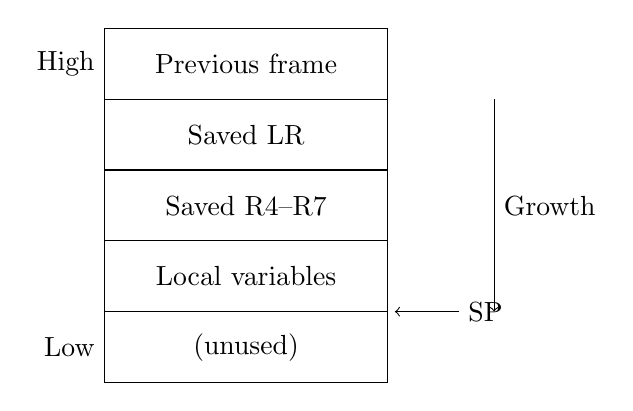
\begin{tikzpicture}[scale=0.9]
    % Stack frame
    \draw (0,0) rectangle (4,5);

    % Divisions
    \draw (0,4) -- (4,4);
    \draw (0,3) -- (4,3);
    \draw (0,2) -- (4,2);
    \draw (0,1) -- (4,1);

    % Labels
    \node at (2,4.5) {Previous frame};
    \node at (2,3.5) {Saved LR};
    \node at (2,2.5) {Saved R4--R7};
    \node at (2,1.5) {Local variables};
    \node at (2,0.5) {(unused)};

    % SP pointer
    \draw[->] (5,1) -- (4.1,1);
    \node[right] at (5,1) {SP};

    % Addresses
    \node[left] at (0,4.5) {High};
    \node[left] at (0,0.5) {Low};

    % Growth arrow
    \draw[->] (5.5,4) -- (5.5,1);
    \node[right] at (5.5,2.5) {Growth};
\end{tikzpicture}
\end{center}

\subsection{PUSH and POP}

\begin{lstlisting}[language=arm]
    @ Save registers to stack
    PUSH  {R4, R5, R6, LR}    @ SP -= 16, store R4,R5,R6,LR

    @ ... function body ...

    @ Restore registers from stack
    POP   {R4, R5, R6, PC}    @ Load R4,R5,R6,PC; SP += 16
                               @ Loading PC = return
\end{lstlisting}

\textbf{PUSH} decrements SP and stores registers (lowest-numbered register at lowest address).

\textbf{POP} loads registers and increments SP. Popping into PC causes a return.

\subsection{ARM Calling Convention (AAPCS)}

The ARM Architecture Procedure Call Standard defines how functions communicate:

\textbf{Arguments}:
\begin{itemize}
    \item First 4 integer/pointer arguments: R0, R1, R2, R3
    \item Additional arguments: pushed on stack (right to left)
    \item Float arguments: S0, S1, S2, ... (up to S15)
\end{itemize}

\textbf{Return values}:
\begin{itemize}
    \item Integer/pointer: R0 (64-bit uses R0:R1)
    \item Float: S0
\end{itemize}

\textbf{Register preservation}:
\begin{itemize}
    \item Caller-saved (scratch): R0--R3, R12, S0--S15
    \item Callee-saved (preserved): R4--R11, S16--S31, SP
    \item LR is overwritten by BL, so callee must save if it calls other functions
\end{itemize}

\subsection{Stack Frame Example}

\begin{center}
\begin{tabular}{p{0.42\textwidth}|p{0.50\textwidth}}
\textbf{C Code} & \textbf{Assembly} \\
\hline
\begin{lstlisting}[language=C, numbers=none]
int compute(int a, int b, int c) {
    int temp1 = a + b;
    int temp2 = b + c;
    int result = temp1 * temp2;
    return result;
}
\end{lstlisting}
&
\begin{lstlisting}[language=arm, numbers=none]
compute:
    @ Args: R0=a, R1=b, R2=c
    @ No need to save regs (no calls)

    ADD   R3, R0, R1   @ temp1 = a + b
    ADD   R0, R1, R2   @ temp2 = b + c
    MUL   R0, R3, R0   @ result = temp1*temp2
    BX    LR           @ Return result
\end{lstlisting}
\end{tabular}
\end{center}

No stack frame needed! The compiler kept everything in registers.

\subsection{Function with Local Array}

\begin{center}
\begin{tabular}{p{0.45\textwidth}|p{0.47\textwidth}}
\textbf{C Code} & \textbf{Assembly} \\
\hline
\begin{lstlisting}[language=C, numbers=none]
int process(int n) {
    int buffer[4];
    for (int i = 0; i < 4; i++) {
        buffer[i] = n + i;
    }
    return buffer[0] + buffer[3];
}
\end{lstlisting}
&
\begin{lstlisting}[language=arm, numbers=none]
process:
    SUB   SP, SP, #16  @ Allocate 16 bytes
    @ buffer at [SP+0..SP+12]

    MOV   R1, #0       @ i = 0
.loop:
    ADD   R2, R0, R1   @ n + i
    STR   R2, [SP, R1, LSL #2]
                       @ buffer[i] = n+i
    ADD   R1, R1, #1
    CMP   R1, #4
    BLT   .loop

    LDR   R0, [SP, #0]  @ buffer[0]
    LDR   R1, [SP, #12] @ buffer[3]
    ADD   R0, R0, R1

    ADD   SP, SP, #16  @ Deallocate
    BX    LR
\end{lstlisting}
\end{tabular}
\end{center}

\subsection{Heap Allocation}

\begin{center}
\begin{tabular}{p{0.45\textwidth}|p{0.47\textwidth}}
\textbf{C Code} & \textbf{Assembly} \\
\hline
\begin{lstlisting}[language=C, numbers=none]
#include <stdlib.h>

int* create_array(int size) {
    int* arr = malloc(size * sizeof(int));
    if (arr != NULL) {
        arr[0] = 42;
    }
    return arr;
}
\end{lstlisting}
&
\begin{lstlisting}[language=arm, numbers=none]
create_array:
    PUSH  {R4, LR}
    LSL   R0, R0, #2   @ size * 4
    BL    malloc       @ Call malloc
    MOV   R4, R0       @ Save pointer

    CMP   R0, #0       @ NULL check
    BEQ   .done
    MOV   R1, #42
    STR   R1, [R0, #0] @ arr[0] = 42

.done:
    MOV   R0, R4       @ Return pointer
    POP   {R4, PC}
\end{lstlisting}
\end{tabular}
\end{center}

\textbf{Heap vs. Stack}:
\begin{itemize}
    \item Stack: Automatic allocation, fixed size, fast
    \item Heap: Dynamic allocation via \texttt{malloc}, variable size, slower
    \item Stack variables deallocated when function returns
    \item Heap variables persist until \texttt{free()} is called
\end{itemize}

%======================================================================
\section{Debugging with Assembly}
%======================================================================

\subsection{Reading a Crash Dump}

When a hard fault occurs, the fault handler can print register values:

\begin{lstlisting}[language=bash]
*** HARD FAULT ***
R0 =0x00000000  R1 =0x20001A3C  R2 =0x00000005  R3 =0xDEADBEEF
R4 =0x200019F0  R5 =0x08004521  R6 =0x00000000  R7 =0x20001A40
R8 =0x00000000  R9 =0x00000000  R10=0x00000000  R11=0x00000000
R12=0x08002345  SP =0x20001A20  LR =0x08003457  PC =0x08002348
xPSR=0x21000000  CFSR=0x00008200
\end{lstlisting}

\textbf{Key values to examine}:
\begin{itemize}
    \item \textbf{PC}: Address where fault occurred---look up in disassembly
    \item \textbf{LR}: Return address---where did we come from?
    \item \textbf{SP}: Stack pointer---is it valid (in SRAM range)?
    \item \textbf{CFSR}: Configurable Fault Status Register---why did we fault?
\end{itemize}

\subsection{Common Fault Patterns}

\begin{center}
\begin{tabular}{lp{8cm}}
\toprule
\textbf{Symptom} & \textbf{Likely Cause} \\
\midrule
PC = 0x00000000 & Called through NULL function pointer \\
PC in 0x20xxxxxx & Jumped into data memory (stack corruption) \\
SP outside SRAM & Stack overflow \\
LR = 0xFFFFFFF9 & Returning from exception (normal) \\
CFSR bit 15 (INVSTATE) & BX to invalid address (bit 0 must be 1 for Thumb) \\
CFSR bit 25 (UNALIGNED) & Unaligned memory access \\
\bottomrule
\end{tabular}
\end{center}

\subsection{Using objdump}

Generate a listing with source code intermixed:

\begin{lstlisting}[language=bash]
arm-none-eabi-objdump -d -S -l firmware.elf > firmware.lst
\end{lstlisting}

\textbf{Flags}:
\begin{itemize}
    \item \texttt{-d}: Disassemble code sections
    \item \texttt{-S}: Intermix source code (requires -g during compilation)
    \item \texttt{-l}: Show line numbers
\end{itemize}

\begin{example}[Finding a Crash Location]
Given PC = \texttt{0x08002348}, search the listing:

\begin{lstlisting}
08002340 <attitude_control>:
attitude_control():
/src/controller.c:42
    float error = setpoint - current;
 8002340:  ee31 0a40   vsub.f32 s0, s2, s0
/src/controller.c:43
    float output = Kp * error;
 8002344:  ee20 0a80   vmul.f32 s0, s0, s1
 8002348:  ed80 0a00   vstr     s0, [r0]    <-- CRASH HERE
\end{lstlisting}

The crash is at a \texttt{vstr} (store float). R0 = 0 means we're storing to address 0---a NULL pointer dereference on line 43 of controller.c.
\end{example}

\subsection{GDB Commands for Assembly}

\begin{lstlisting}[language=bash]
# Connect to target
arm-none-eabi-gdb firmware.elf
(gdb) target remote :3333

# Disassemble current function
(gdb) disassemble

# Show next 10 instructions
(gdb) x/10i $pc

# Show all registers
(gdb) info registers
(gdb) info registers s0 s1 s2    # FPU registers

# Single-step one instruction
(gdb) stepi

# Step over function call
(gdb) nexti

# Set breakpoint at address
(gdb) break *0x08002348

# Examine memory
(gdb) x/4xw 0x20001000   # 4 words in hex
(gdb) x/s 0x20001000     # as string
\end{lstlisting}

%======================================================================
\section{Performance Considerations}
%======================================================================

\subsection{Instruction Cycle Counts}

Most Cortex-M4 instructions execute in 1 cycle, but some take longer:

\begin{center}
\begin{tabular}{llp{5cm}}
\toprule
\textbf{Operation} & \textbf{Cycles} & \textbf{Notes} \\
\midrule
MOV, ADD, SUB, AND, ORR & 1 & Register operations \\
MUL & 1 & 32-bit multiply \\
SDIV, UDIV & 2--12 & Division (operand-dependent) \\
LDR (from SRAM) & 1--2 & May stall on bus contention \\
LDR (from Flash) & 1--5 & Flash wait states (depends on speed) \\
VADD.F32, VMUL.F32 & 1 & FPU operations \\
VMLA.F32 & 1 & Multiply-accumulate \\
VDIV.F32 & 14 & Floating-point division \\
VSQRT.F32 & 14 & Square root \\
B (taken) & 1--3 & Pipeline flush \\
BL (function call) & 1--3 & Plus function prologue overhead \\
\bottomrule
\end{tabular}
\end{center}

\begin{keyidea}[title=Avoid Division and Square Root]
Division and square root are 14$\times$ slower than multiplication. In inner loops:
\begin{itemize}
    \item Replace \texttt{x / constant} with \texttt{x * (1/constant)}
    \item Precompute reciprocals outside the loop
    \item Use \texttt{rsqrt} approximations if precision allows
\end{itemize}
\end{keyidea}

\subsection{Pipeline Effects}

The Cortex-M4 has a 3-stage pipeline (Fetch, Decode, Execute). Branch instructions can cause a \textbf{pipeline flush}---the fetched/decoded instructions are discarded.

\textbf{Branch prediction}: Cortex-M4 has limited branch prediction. Conditional branches that are usually taken have lower cost than unpredictable branches.

\textbf{Loop optimization}: Small loops that fit in the prefetch buffer execute efficiently.

\subsection{Memory Access Patterns}

\begin{itemize}
    \item \textbf{Sequential access}: Fast---prefetch works well
    \item \textbf{Strided access}: Slower---prefetch less effective
    \item \textbf{Random access}: Slowest---no prefetch benefit
\end{itemize}

For array processing, access elements sequentially when possible:
\begin{lstlisting}[language=C]
// Good: Sequential access
for (int i = 0; i < N; i++) {
    sum += arr[i];
}

// Bad: Strided access (if avoidable)
for (int i = 0; i < N; i += 4) {
    sum += arr[i];
}
\end{lstlisting}

\subsection{Compiler Optimization}

The compiler applies many optimizations automatically:

\begin{itemize}
    \item \textbf{Strength reduction}: \texttt{x * 4} becomes \texttt{x << 2}
    \item \textbf{Common subexpression elimination}: Compute shared values once
    \item \textbf{Loop unrolling}: Reduce branch overhead by doing multiple iterations per loop cycle
    \item \textbf{Inlining}: Replace function call with function body
    \item \textbf{Register allocation}: Keep frequently-used variables in registers
\end{itemize}

\textbf{Optimization flags}:
\begin{itemize}
    \item \texttt{-O0}: No optimization (for debugging)
    \item \texttt{-O2}: Standard optimization (recommended)
    \item \texttt{-O3}: Aggressive optimization (may increase code size)
    \item \texttt{-Os}: Optimize for size
\end{itemize}

\begin{example}[Compiler-Optimized PID Loop]
\begin{lstlisting}[language=C]
float pid_update(PID* pid, float error, float dt) {
    pid->integral += error * dt;
    float derivative = (error - pid->prev_error) / dt;
    pid->prev_error = error;
    return pid->Kp * error + pid->Ki * pid->integral + pid->Kd * derivative;
}
\end{lstlisting}

With \texttt{-O2}, the compiler will:
\begin{enumerate}
    \item Keep \texttt{error} and \texttt{dt} in FPU registers
    \item Use VMLA for the multiply-accumulate operations
    \item Precompute \texttt{1/dt} if it detects \texttt{dt} is constant
    \item Potentially inline this function at call sites
\end{enumerate}
\end{example}

\section{Chapter Summary}

This appendix introduced ARM Cortex-M4 architecture and assembly language:

\begin{itemize}
    \item \textbf{Architecture}: The STM32F405 contains a Cortex-M4F core running at 168 MHz with hardware FPU, 1 MB Flash, and 192 KB SRAM.

    \item \textbf{Registers}: 16 general-purpose registers (R0--R15), with R13 (SP), R14 (LR), and R15 (PC) having special roles. The FPU adds 32 single-precision registers (S0--S31).

    \item \textbf{Instruction set}: ARM Thumb-2 provides efficient 16/32-bit mixed instructions. Key categories include data movement (MOV, LDR, STR), arithmetic (ADD, SUB, MUL), logic (AND, ORR), comparison (CMP), and branching (B, BL, BX).

    \item \textbf{Function calls}: The AAPCS defines argument passing (R0--R3), return values (R0), and register preservation conventions that enable interoperable code.

    \item \textbf{Debugging}: Understanding assembly is essential for interpreting crash dumps, using GDB effectively, and tracing bugs to source code.

    \item \textbf{Performance}: Most instructions take 1 cycle, but division (2--12 cycles) and FPU division/sqrt (14 cycles) are slow. The compiler handles most optimization automatically.
\end{itemize}

\begin{keyidea}[title=The Essential Skill]
You don't need to write assembly, but you do need to read it. When your quadrotor crashes, the CPU gives you a PC value. Your job is to trace that back through the disassembly to your C code and understand what went wrong.
\end{keyidea}
\index{ARM architecture|)}
\index{assembly language|)}
